\textbf{Reactive feedback.} Transformers were used to increase the input matching feedback and bandwidth while adding as little as possible additional noise \cite{FDSOI2}. Figure \ref{fig:FDSOI:TRX:LNA_REACTIVE_FEEDBACK} shows a small-signal equivalent of figure \ref{fig:FDSOI:TRX:LNA} demonstrating how the series-shunt feedback is achieved. Taking into consideration the direction of currents and the dot rule we get the following system of equations.
			\begin{equation}\label{eq:FDSOI:Transformer_voltages}
				\begin{bNiceMatrix}
					v_{\symup{in}}\\
					v_{L_{dl}}\\
					v_{L_{dr}}
				\end{bNiceMatrix}=\begin{bNiceMatrix}
					L_g & M_1 & -M_1 \\
					M_1 & L_{dl} & -M_2 \\
					-M_1 & -M_2 & L_{dr}
				\end{bNiceMatrix} \begin{bNiceMatrix}
					\nicefrac{d i_{L_{g}}}{dt}\\
					\nicefrac{d i_{L_{dl}}}{dt}\\
					\nicefrac{d i_{L_{dr}}}{dt}
				\end{bNiceMatrix},
			\end{equation}
			where $M_1=k_1\sqrt{L_g L_{dl}}=k_1\sqrt{L_g L_{dr}}$ is the mutual inductance between coils $L_g-L_{dl}$ and $L_g-L_{dr}$, and $M_2=k_2\sqrt{L_{dl} L_{dr}}=k_1L_{dl}$ is the mutual inductunce between coils $L_{dl}-L_{dr}$. $L_{dr}$ and $L_{dl}$ are identical.\par
			The authors report that the real part of the input resistance of the single-ended LNA can be approximated by \eqref{eq:FDSOI:Rin_single_ended_LNA}
			\begin{equation}\label{eq:FDSOI:Rin_single_ended_LNA}
				\RE{\left( Z_{\symup{in}} \right)}\approxeq \frac{N_g}{k_1 g_m^{\text{\tiny{(11)}}}},
			\end{equation}
			where $N_g=n_{L_g}\cdot n_{L_{dl}}^{-1}$ is the turn ratio of the input transformer, $k_1\to 1$ is their coupling coefficient and $g_{m}^{\text{\tiny{(11)}}}$ is the transconductance of the input transistor.\par
			The single-turn windings, $L_{dl}$ and $L_{dr}$, are intertwined \cite{FDSOI2}. The secondary winding, $L_g$, consists of seven turns and is placed on top of the primary ones \cite{FDSOI2}. The transformer is integrated on the chip. A three-dimensional representation of the windings' configuration is shown in figure \ref{fig:FDSOI:LNA:transformers}.

			\begin{figure}[ht!]
				\centering
				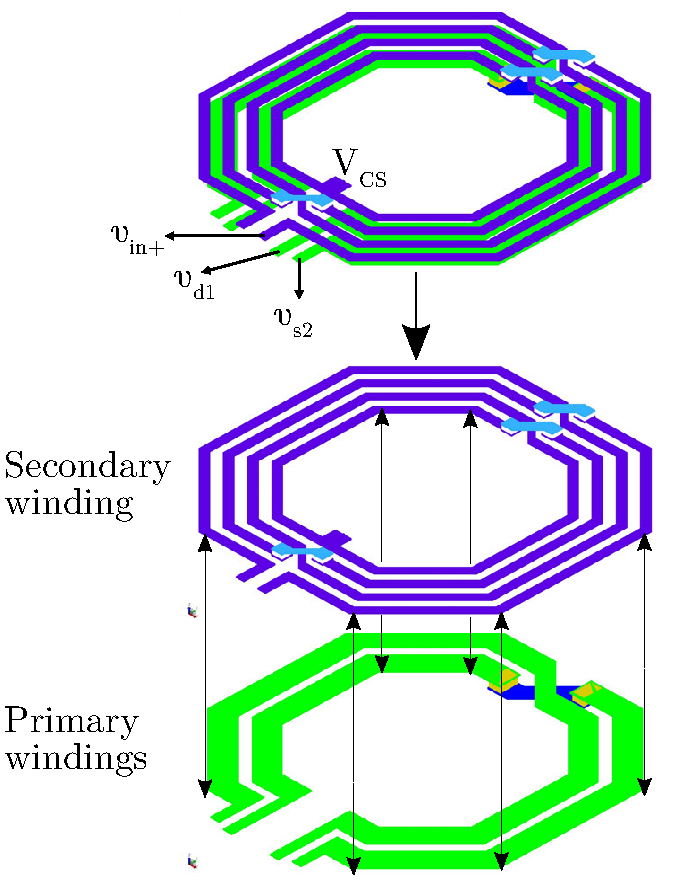
\includegraphics[width=0.6\linewidth]{assets/FD-SOI/Sub_6GHz_TRX_assets/LNA_inductors.pdf}
				\caption{Three-dimensional representation of the transformer used in the LNA of figure \ref{fig:FDSOI:TRX:LNA}. Figure taken from \cite{FDSOI2}.}
				\label{fig:FDSOI:LNA:transformers}
			\end{figure}